\chapter{ບົດນຳສະເໜີ}

\section{ຄວາມເປັນມາ}
ຂຽນອະທິບາຍພື້ນຫຼັງ ຄວາມສຳຄັນ ແລະ ເຫດຜົນທີ່ເລືອກຫົວຂໍ້ນີ້. ນຳສະເໜີສະພາບປັດຈຸບັນ ບັນຫາທີ່ພົບ ແລະ ຄວາມຈຳເປັນໃນການພັດທະນາໂຄງການ. ຕົວຢ່າງການອ້າງອີງແບບຕົວເລກແມ່ນ \cite{lamport1994latex}.

\section{ບັນຫາຂອງການສຶກສາ}
ລະບຸບັນຫາຫຼັກ ແລະ ບັນຫາຍ່ອຍທີ່ໂຄງການຈະແກ້ໄຂ. ຄວນຂຽນໃຫ້ຊັດເຈນ ວັດແທກໄດ້ ແລະ ເຊື່ອມກັບຈຸດປະສົງ.

\section{ຈຸດປະສົງຂອງການສຶກສາ}
\begin{enumerate}
  \item ເພື່ອສຶກສາ ວິເຄາະ ແລະ ອອກແບບລະບົບຕາມຫົວຂໍ້ໂຄງການ.
  \item ເພື່ອພັດທະນາຕົ້ນແບບ ຫຼື ລະບົບທີ່ສາມາດນຳໃຊ້ໄດ້.
  \item ເພື່ອທົດສອບ ແລະ ປະເມີນຜົນການໃຊ້ງານຂອງລະບົບ.
\end{enumerate}

\section{ຄຳຖາມການຄົ້ນຄວ້າ}
\begin{enumerate}
  \item ລະບົບທີ່ພັດທະນາສາມາດແກ້ບັນຫາທີ່ກຳນົດໄດ້ຫຼືບໍ່?
  \item ຜູ້ໃຊ້ມີຄວາມພຶງພໍໃຈຕໍ່ລະບົບໃນລະດັບໃດ?
\end{enumerate}

\section{ຂອບເຂດການສຶກສາ}
ລະບຸຂອບເຂດດ້ານເນື້ອຫາ ຜູ້ໃຊ້ ອຸປະກອນ ຊອບແວ ເວລາ ແລະ ສິ່ງທີ່ບໍ່ຢູ່ໃນຂອບເຂດໂຄງການ.

\section{ປະໂຫຍດທີ່ຄາດວ່າຈະໄດ້ຮັບ}
\begin{enumerate}
  \item ໄດ້ລະບົບ ຫຼື ຕົ້ນແບບທີ່ສາມາດນຳໄປສຶກສາ ແລະ ພັດທະນາຕໍ່ໄດ້.
  \item ຊ່ວຍແກ້ບັນຫາ ຫຼື ປັບປຸງກະບວນການໃນຂອບເຂດທີ່ສຶກສາ.
\end{enumerate}

\section{ໂຄງສ້າງຂອງບົດ}
ບົດທີ 1 ນຳສະເໜີພາບລວມຂອງໂຄງການ. ບົດທີ 2 ນຳສະເໜີທິດສະດີ ແລະ ງານທີ່ກ່ຽວຂ້ອງ. ບົດທີ 3 ອະທິບາຍວິທີດຳເນີນງານ. ບົດທີ 4 ສະແດງຜົນ ແລະ ອະພິປາຍຜົນ. ບົດທີ 5 ສະຫຼຸບ ແລະ ສະເໜີແນະ.

\begin{table}[H]
\centering
\caption{ສະແດງແຜນການດຳເນີນງານ}
\label{tab:sample-plan}
\begin{tabularx}{\textwidth}{>{\centering\arraybackslash}p{1.2cm}X>{\centering\arraybackslash}p{2.5cm}}
\toprule
\textbf{ລຳດັບ} & \textbf{ກິດຈະກຳ} & \textbf{ໄລຍະເວລາ}\\
\midrule
1 & ສຶກສາເອກະສານ ແລະ ວິເຄາະບັນຫາ & 2 ອາທິດ\\
2 & ອອກແບບລະບົບ ແລະ ຖານຂໍ້ມູນ & 3 ອາທິດ\\
3 & ພັດທະນາ ແລະ ທົດສອບ & 6 ອາທິດ\\
\bottomrule
\end{tabularx}
\end{table}


\begin{figure}[H]
  \centering
  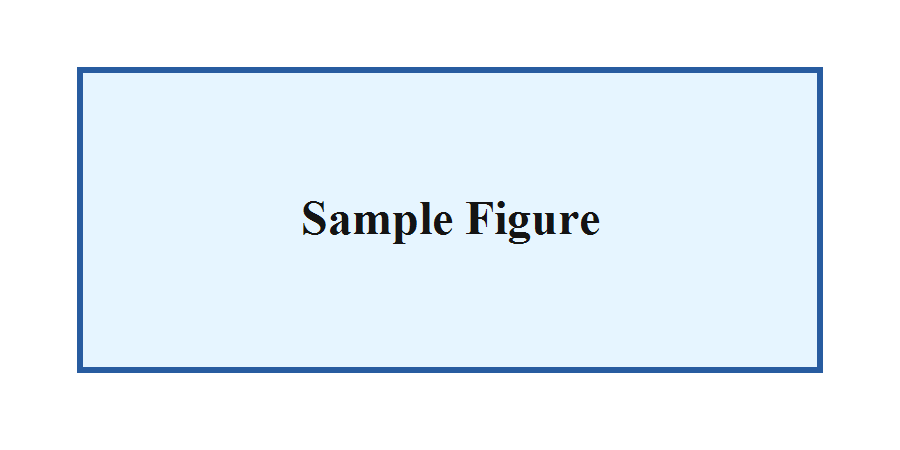
\includegraphics[width=0.65\textwidth]{figures/sample-figure.png}
  \caption{ຕົວຢ່າງການໃສ່ຮູບໃນບົດ}
  \label{fig:sample}
\end{figure}

ຕົວຢ່າງການອ້າງຮູບແມ່ນ ຮູບທີ~\ref{fig:sample} ແລະ ຕົວຢ່າງການອ້າງຕາຕະລາງແມ່ນ ຕາຕະລາງທີ~\ref{tab:sample-plan}.
